\documentclass[journal,12pt,twocolumn]{IEEEtran}

\usepackage[utf8]{inputenc}
\usepackage{kvmap}
\usepackage{graphics} 

\usepackage{setspace}
\usepackage{gensymb}

\singlespacing




\usepackage{amsthm}

\usepackage{mathrsfs}
\usepackage{txfonts}
\usepackage{stfloats}
\usepackage{bm}
\usepackage{cite}
\usepackage{cases}
\usepackage{subfig}

\usepackage{longtable}
\usepackage{multirow}

\usepackage{enumitem}
\usepackage{mathtools}
\usepackage{steinmetz}
\usepackage{tikz}
\usepackage{circuitikz}
\usepackage{verbatim}
\usepackage{tfrupee}
\usepackage[breaklinks=true]{hyperref}
\usepackage{graphicx}
\usepackage{tkz-euclide}
\usepackage{float}

\usetikzlibrary{calc,math}
\usepackage{listings}
    \usepackage{color}                                            %%
    \usepackage{array}                                            %%
    \usepackage{longtable}                                        %%
    \usepackage{calc}                                             %%
    \usepackage{multirow}                                         %%
    \usepackage{hhline}                                           %%
    \usepackage{ifthen}                                           %%
    \usepackage{lscape}     
\usepackage{multicol}
\usepackage{chngcntr}

\DeclareMathOperator*{\Res}{Res}

\renewcommand\thesection{\arabic{section}}
\renewcommand\thesubsection{\thesection.\arabic{subsection}}
\renewcommand\thesubsubsection{\thesubsection.\arabic{subsubsection}}

\renewcommand\thesectiondis{\arabic{section}}
\renewcommand\thesubsectiondis{\thesectiondis.\arabic{subsection}}
\renewcommand\thesubsubsectiondis{\thesubsectiondis.\arabic{subsubsection}}


\hyphenation{op-tical net-works semi-conduc-tor}
\def\inputGnumericTable{}                                 %%

\lstset{
%language=C,
frame=single, 
breaklines=true,
columns=fullflexible
}
\begin{document}


\newtheorem{theorem}{Theorem}[section]
\newtheorem{problem}{Problem}
\newtheorem{proposition}{Proposition}[section]
\newtheorem{lemma}{Lemma}[section]
\newtheorem{corollary}[theorem]{Corollary}
\newtheorem{example}{Example}[section]
\newtheorem{definition}[problem]{Definition}

\newcommand{\BEQA}{\begin{eqnarray}}
\newcommand{\EEQA}{\end{eqnarray}}
\newcommand{\define}{\stackrel{\triangle}{=}}
\newcommand\hlight[1]{\tikz[overlay, remember picture,baseline=-\the\dimexpr\fontdimen22\textfont2\relax]\node[rectangle,fill=blue!50,rounded corners,fill opacity = 0.2,draw,thick,text opacity =1] {$#1$};}
\bibliographystyle{IEEEtran}
\providecommand{\mbf}{\mathbf}
\providecommand{\pr}[1]{\ensuremath{\Pr\left(#1\right)}}
\providecommand{\qfunc}[1]{\ensuremath{Q\left(#1\right)}}
\providecommand{\sbrak}[1]{\ensuremath{{}\left[#1\right]}}
\providecommand{\lsbrak}[1]{\ensuremath{{}\left[#1\right.}}
\providecommand{\rsbrak}[1]{\ensuremath{{}\left.#1\right]}}
\providecommand{\brak}[1]{\ensuremath{\left(#1\right)}}
\providecommand{\lbrak}[1]{\ensuremath{\left(#1\right.}}
\providecommand{\rbrak}[1]{\ensuremath{\left.#1\right)}}
\providecommand{\cbrak}[1]{\ensuremath{\left\{#1\right\}}}
\providecommand{\lcbrak}[1]{\ensuremath{\left\{#1\right.}}
\providecommand{\rcbrak}[1]{\ensuremath{\left.#1\right\}}}
\theoremstyle{remark}
\newtheorem{rem}{Remark}
\newcommand{\sgn}{\mathop{\mathrm{sgn}}}
\providecommand{\abs}[1]{\left\vert#1\right\vert}
\providecommand{\res}[1]{\Res\displaylimits_{#1}} 
\providecommand{\norm}[1]{$\left\lVert#1\right\rVert$}
%\providecommand{\norm}[1]{\lVert#1\rVert}
\providecommand{\mtx}[1]{\mathbf{#1}}
\providecommand{\mean}[1]{E\left[ #1 \right]}
\providecommand{\fourier}{\overset{\mathcal{F}}{ \rightleftharpoons}}
%\providecommand{\hilbert}{\overset{\mathcal{H}}{ \rightleftharpoons}}
\providecommand{\system}{\overset{\mathcal{H}}{ \longleftrightarrow}}
	%\newcommand{\solution}[2]{\textbf{Solution:}{#1}}
\newcommand{\solution}{\noindent \textbf{Solution: }}
\newcommand{\cosec}{\,\text{cosec}\,}
\providecommand{\dec}[2]{\ensuremath{\overset{#1}{\underset{#2}{\gtrless}}}}
\newcommand{\myvec}[1]{\ensuremath{\begin{pmatrix}#1\end{pmatrix}}}
\newcommand{\mydet}[1]{\ensuremath{\begin{vmatrix}#1\end{vmatrix}}}
\numberwithin{equation}{subsection}
\makeatletter
\@addtoreset{figure}{problem}
\makeatother
\let\StandardTheFigure\thefigure
\let\vec\mathbf
\renewcommand{\thefigure}{\theproblem}
\def\putbox#1#2#3{\makebox[0in][l]{\makebox[#1][l]{}\raisebox{\baselineskip}[0in][0in]{\raisebox{#2}[0in][0in]{#3}}}}
     \def\rightbox#1{\makebox[0in][r]{#1}}
     \def\centbox#1{\makebox[0in]{#1}}
     \def\topbox#1{\raisebox{-\baselineskip}[0in][0in]{#1}}
     \def\midbox#1{\raisebox{-0.5\baselineskip}[0in][0in]{#1}}
\vspace{3cm}

\title{Assignment No.1}

\author{Dukkipati Vijay Sai}
\maketitle
\newpage
\bigskip
\renewcommand{\thefigure}{\theenumi}
\renewcommand{\thetable}{\theenumi}


Download IDE code from 
\begin{lstlisting}
https://github.com/dukkipativijay/Fwciith2022/blob/main/Assignment1.cpp
\end{lstlisting}
Download Assembly code from
\begin{lstlisting}
https://github.com/dukkipativijay/Fwciith2022/tree/main/Assignment%201/Codes/asm
\end{lstlisting}
Download GCC code from
\begin{lstlisting}
https://github.com/dukkipativijay/Fwciith2022/blob/main/Assignment%201%20-%20GCC/main.c
\end{lstlisting}
%
and latex-tikz codes from 
%
\begin{lstlisting}
https://github.com/dukkipativijay/Fwciith2022/blob/main/Assignment%201/Latex%20File.tex
\end{lstlisting}
%
\section{Question-2016 Section C Q6(d)}

Reduce the following Boolean Expression to its simplest form using k-map
$F=(X,Y,Z,W)= \sum(2,6,7,8,9,10,11,13,14,15)$
\section{Contents}
\raggedright
\textbf{Components}
\hspace{10em} 3
\\\textbf{Hardware}
\hspace{11em} 4
\\\textbf{Solution}
\hspace{11.8em}   5\\
\textit{Abstract-}
\textbf{This manual shows how to use 7447 BCD-seven segment display encoder to display Boolean Logic}
\section{Components}
\centering
\begin{tabular}{|l|c|c|}
\hline
Component & Value & Quantity\\
\hline
Resistor & 220 Ohm & 1\\
\hline
Arduino & UNO & 1\\
\hline
Seven Segment Display & & 1\\
\hline
Decoder & 7447 & 1\\
\hline
Jumper Wires & M-M & 20\\
\hline
Breadboard & & 1\\
\hline
\end{tabular}\\
\
\centerline{Table 3.0}

\section{Hardware}
\raggedright
Make connections between seven segment display and the 7447 ic as per the given table\\
\
\centering
\\\begin{tabular}{|l|c|c|c|c|c|c|c|}
\hline
\textbf{7447} & a' & b' & c' & d' & e' & f' & g'\\
\hline
\textbf{Display} & a & b & c & d & e & f & g\\
\hline
\end{tabular}\\
\
\centerline{Table 4.0}


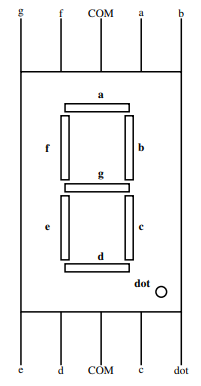
\includegraphics{ss fig.png}
\begin{center}
\textbf{Figure 1}
\end{center}

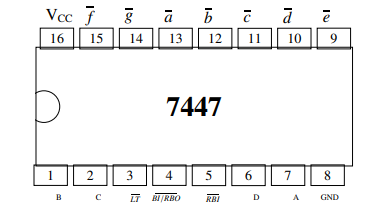
\includegraphics{ic fig.png}
\begin{center}

\textbf{Figure 2} \\

\end{center}
\centering

\begin{tabular}{|l|c|c|c|c|}
\hline
\textbf{7447} & D & C & B & A\\
\hline
\textbf{Arduino} & 5 & 4 & 3 & 2\\
\hline
\end{tabular}\\
\
\centerline{Table 4.1}\\

\centering
\begin{tabular}{|l|c|c|c|c|}
\hline
& X & Y & Z & W\\
\hline
\textbf{Input} & 0 & 1 & 1 & 0\\
\hline
\textbf{Arduino} & 6 & 7 & 8 & 9\\
\hline
\end{tabular}\\

\centerline{Table 4.2}
In the above example we are taking number 6 as input to the arduino and displaying 1 on the seven segment display.

\section{Solution} 
\centering
\textbf{Truth Table}\\
\begin{tabular}{|c|c|c|c||c|}
\hline
\textbf{X} & \textbf{Y} & \textbf{Z} & \textbf{W} & \textbf{F}\\
\hline
0 & 0 & 0 & 0 & 0\\
\hline
0 & 0 & 0 & 1 & 0\\
\hline
0 & 0 & 1 & 0 & 1\\
\hline
0 & 0 & 1 & 1 & 0\\
\hline
0 & 1 & 0 & 0 & 0\\
\hline
0 & 1 & 0 & 1 & 0\\
\hline
0 & 1 & 1 & 0 & 1\\
\hline
0 & 1 & 1 & 1 & 1\\
\hline
1 & 0 & 0 & 0 & 1\\
\hline
1 & 0 & 0 & 1 & 1\\
\hline
1 & 0 & 1 & 0 & 1\\
\hline
1 & 0 & 1 & 1 & 1\\
\hline
1 & 1 & 0 & 0 & 0\\
\hline
1 & 1 & 0 & 1 & 1\\
\hline
1 & 1 & 1 & 0 & 1\\
\hline
1 & 1 & 1 & 1 & 1\\
\hline
\end{tabular}\\
\
\centerline{Table 5.0}
\centering
\begin{kvmap}
    \begin{kvmatrix}{Z,W,X,Y}
    0 & 0 & 0 & 1\\
    0 & 0 & 1 & 1\\
    0 & 1 & 1 & 1\\
    1 & 1 & 1 & 1\\
    \end{kvmatrix}
    \bundle[color=red]{0}{3}{3}{3}
    
\end{kvmap}
\
\centerline{Table 5.1}

\raggedright{The expression in the above k-map results in XY'}
\centering
\begin{kvmap}
    \begin{kvmatrix}{Z,W,X,Y}
    0 & 0 & 0 & 1\\
    0 & 0 & 1 & 1\\
    0 & 1 & 1 & 1\\
    1 & 1 & 1 & 1\\
    \end{kvmatrix}
    \bundle[color=blue]{1}{2}{2}{3}
\end{kvmap}\\

\centerline{Table 5.2}
\raggedright{The expression in the above map k-map results in XW}\\
\centering

\begin{kvmap}
    \begin{kvmatrix}{Z,W,X,Y}
    0 & 0 & 0 & 1\\
    0 & 0 & 1 & 1\\
    0 & 1 & 1 & 1\\
    1 & 1 & 1 & 1\\
    \end{kvmatrix}
    \bundle[color=violet]{2}{2}{3}{3}
\end{kvmap}\\
\centerline{Table 5.3}
\raggedright{The expression in the above map k-map results in XZ}\\
\centering
\begin{kvmap}
    \begin{kvmatrix}{Z,W,X,Y}
    0 & 0 & 0 & 1\\
    0 & 0 & 1 & 1\\
    0 & 1 & 1 & 1\\
    1 & 1 & 1 & 1\\
    \end{kvmatrix}
    \bundle[color=cyan]{2}{1}{3}{2}
\end{kvmap}\\
\centerline{Table 5.4}
\raggedright{The expression in the above k-map results in YZ}
\centering
\begin{kvmap}
    \begin{kvmatrix}{Z,W,X,Y}
    0 & 0 & 0 & 1\\
    0 & 0 & 1 & 1\\
    0 & 1 & 1 & 1\\
    1 & 1 & 1 & 1\\
    \end{kvmatrix}
    \bundle[color=black]{3}{0}{3}{3}
\end{kvmap}\\
\centerline{Table 5.5}
\raggedright{The expression in the above k-map results in ZW'}\\
\ 

\raggedright

By solving the above Karnaugh Map, we get the simplified boolean expression given below\\
\centering

$$F=XY'+XW+XZ+YZ+ZW'$$


\end{document}

Footer
